\documentclass[10pt, twoside]{book}
    \usepackage[italian]{babel}
    \usepackage[utf8]{inputenc}
    \usepackage[T1]{fontenc}
%%%%% Pacchetti
\usepackage{FileAusiliari/Layout}			% Contiene i pacchetti e le impostazioni per il layout
\usepackage{FileAusiliari/Pacchetti}		% Pacchetti aggiuntivi di vario tipo (senza tikz)
\usepackage{FileAusiliari/TikZ}				% Ambiente tikzpicture
\usepackage{FileAusiliari/Definizioni}		% Definizioni di colori, variabili globali ecc.
\usepackage{FileAusiliari/Environments}		% Impostazioni TOC, bibliografia e indice analitico + environments vari per il contenuto del documento
\usepackage{FileAusiliari/Custom}			% Tutto ciò che è personalizzabile normalmente dall'utente (tranne i colori per collegamenti ipertestuali, citazioni, link, che sono da modificare in Referencing)
%%%%%%%%%% Impostazioni indice analitico
%%%%%%%%%%%%%%%%%%%%%%%%%%%%%%%%%%%%
\usepackage{imakeidx}
\indexsetup{othercode=\small}
\makeindex[columns=2, intoc=false, columnseprule, title={}, 
           options= -s FileAusiliari/Stile.ist]
%%%%%%%%%%									Collegamenti ipertestuali
%%%%%%%%%%
\RequirePackage[breaklinks, colorlinks=true, hypertexnames=true, linktoc=all]{hyperref}

	%%%%%%%%%% Colori dei link ipertestuali
	\hypersetup{colorlinks, %I colori sono per il pdf, per la stampa impostare 'black' per tutti i colori
			urlcolor={Url},  % default='Url'
			citecolor={Cite}, % default='Cite'
			linkcolor={Link}} % default='Link'

%%% Miglior referencing
\pagenumbering{none}		% Collegamenti ipertestuali e indice analitico
\usepackage{FileAusiliari/Comandi}			% Comandi vari
\usepackage{fancyhdr}
\usepackage{titlesec}
\usepackage{listings}
\usepackage{graphicx}
\usepackage{caption}
\usepackage{hyperref}
\usepackage{makeidx}
\usepackage{xcolor}


\usepackage{fontspec} % 字體
\usepackage{xeCJK}    % 中文支持
\setmainfont{Times New Roman} % 主字體
\setCJKmainfont{Noto Sans CJK TC} % 中文黑體 思源黑體
\linespread{1.5}

\newcommand{\CJKsection}[1]{{\CJKfamily{titlefont}#1}} % 中文支持 Section Title
\titleformat{\section}{\Large\bfseries\CJKsection}{\thesection}{1em}{}

% 自定義命令
\newcommand{\code}[1]{\texttt{#1}}
\newcommand{\term}[1]{\textit{#1}}
\renewcommand{\bold}[1]{\textbf{#1}}
\newcommand{\figref}[1]{\textbf{Figure~\ref{#1}}}
\newcommand{\tabref}[1]{\textbf{Table~\ref{#1}}}
\newcommand{\lstref}[1]{\textbf{Listing~\ref{#1}}}
\newcommand{\chapref}[1]{\textbf{Chapter~\ref{#1}}}
\newcommand{\secref}[1]{\textbf{Section~\ref{#1}}}



%%%%%%%%%%%%%%%%%%%%%%%%%%%%
%%%%%%%%%%%%%%%%%%%%%%%%%%%%
\begin{document}
%%%%%%%%%%%%%%%%%%%%%%%%%%%%									 TITOLO
%%%%%%%%%%%%%%%%%%%%%%%%%%%%
% \begin{titlepage}
    \raggedleft	
    \rule{1pt}{.125\textheight}
	\hspace{0.025\textwidth}
	\parbox[b]{.85\textwidth}{
		{\HUGE\bfseries Titolo (versione 1)
        }\\[2\baselineskip]
		{\Large\textit{Sottotitolo}}\\[45.5\baselineskip]
        {\Large\textsc{Mattia Puddu}\\[.35\baselineskip] mattiapuddu@icloud.com} \\\\\\\\
        %{\Large\textit{Mattia Puddu (seconda versione)}}\\
        {\Large\today}

 }
\end{titlepage}
\begin{titlepage}

% % LOGO
% \begin{figure}[ht]\centering
%     
\includegraphics[scale=.6]{FileAusiliari/Logo/MarchioBlack.pdf}
% \end{figure}

% TITLE AND SUBTITLE
\vspace{2.5cm}
\parbox[l]{.9\textwidth}{\centering
    {\HUGE \bfseries 使用 HIP 的加速運算}\\[2\baselineskip]
    {\Large \textit{加速運算技術與應用研究}}\\[.5\baselineskip]}

\vspace*{\fill}

% AUTHOR
\parbox[b]{.5\textwidth}{
    \rule{1pt}{.125\textheight}
    \hspace{0.025\textwidth}
    \parbox[b]{.8\textwidth}{
        {\Large \bfseries 作者}\\[1\baselineskip]
        {\Large \textsc{Yifan Sun, Sabila Al Jannat, \\ Trinayan Baruah, and David Kaeli}}\\[2\baselineskip]
        {\Large 2024 年 10 月}
    }
}
\parbox[b]{.5\textwidth}{
    \rule{1pt}{.125\textheight}
    \hspace{0.025\textwidth}
    \parbox[b]{.8\textwidth}{
        {\Large \bfseries 翻譯}\\[1\baselineskip]
        {\Large \textsc{牟展佑、程詩柔、謝之豫、牟懋軒\\林展毅、黃煒智、魏士勛、白宸安\\郭品毅、周志遠}}\\[1\baselineskip]
        {\Large 2025 年 7 月}
    }
}
\end{titlepage}

%%%%%%%%%%%%%%%%%%%%%%%%%%%%									FRONTMATTER
%%%%%%%%%%%%%%%%%%%%%%%%%%%%
\frontmatter
\pagestyle{fancyfront}
%%%%%								 INDICE
\begingroup
{
	\let\cleardoublepage\relax
	%%%%%		Nome Indice (NASCOSTO E CREATO A PARTE)
	\renewcommand\contentsname{}
	\begin{tikzpicture}[remember picture, overlay]
		\clip (-80,-95) rectangle (40,10);
		\pgftext[x=.8\textwidth, y=0.2cm]{\HUGE\bfseries 
		Indice}						% Titolo indice
		\end{tikzpicture}
	\vspace{-1cm}
	
	\tableofcontents
	\vspace{.25cm}
}
%%%%%								INTRODUZIONE
		\titleformat{\chapter}
		[hang]
		{\Huge}
		{}
		{0em}
		{}
		[\Large {\begin{tikzpicture} [remember picture, overlay]
		\pgftext[right,x=14.75cm,y=0.2cm]{\HUGE\bfseries 
			前言}
		\end{tikzpicture}}]
%%%%%%%%%%%%%%%%%%%%%%%%%%%%%%%%%%%%%%%%%%%%%%%%%%%%%%%%%%%%%%%%%%%%%%%%%%%%%%%%%
\chapter*{}\normalfont\addcontentsline{toc}{part}{前言}

高效能運算(High-Performance Computing, HPC)的世界最近見證了一個重要里程碑,即在美國橡樹嶺國家實驗室(Oak Ridge National Laboratory)部署的 \textbf{Frontier 超級電腦}首次達成 \textbf{Exascale} 性能。隨著計算性能的此項突破,一類全新的應用場景得以實現,包括:
\begin{itemize}
    \item 天氣與氣候預測,
    \item 生物醫學研究,
    \item 高端設備開發,
    \item 新能源研究與探索,
    \item 動畫設計,
    \item 新材料研究,
    \item 工程設計、模擬與分析,
    \item 遙測數據處理,以及
    \item 金融風險分析。
\end{itemize}

\textbf{AMD} 透過提供一系列高效能的 \textbf{CPU} 和 \textbf{GPU},以及支持 \textbf{HIP} 和 \textbf{ROCm} 執行的開源軟體堆棧,推動了這些進展的實現。這個新興的程式設計生態系統提供了許多創新的功能,包括硬體加速器(如 \textbf{AMD} 和 \textbf{NVIDIA GPU})的互操作性,以及對關鍵高效能編譯器(如 \textbf{LLVM})、叢集部署及核心應用框架(如 \textbf{Raja}、\textbf{Kokkos}、\textbf{TensorFlow} 和 \textbf{PyTorch})的支持,還包含多項高效能函式庫(如 \textbf{rocBLAS}、\textbf{rocSparse}、\textbf{MIOpen}、\textbf{RCCL} 和 \textbf{rocFFT})。

為配合這些進步,高效能運算社群也對此里程碑作出了貢獻,提供了最先進的第三方工具,用於性能監控、除錯器,以及視覺化工具。

由 \textbf{Yifan Sun}、\textbf{Sabila Al Jannat}、\textbf{Trinayan Baruah} 和 \textbf{David Kaeli} 共同撰寫的《\textit{Accelerated Computing with HIP}》第二版,為高效能運算社群提供了一份具參考價值的指南,幫助程式開發人員充分利用 \textbf{Exascale} 計算的優勢。該書內容涵蓋以下主題:


		\titleformat{\chapter}
		[hang]
		{\Huge}
		{}
		{0em}
		{}
		[\Large {\begin{tikzpicture} [remember picture, overlay]
		\pgftext[right,x=14.75cm,y=0.2cm]{\HUGE\bfseries 
			書寫規範}
		\end{tikzpicture}}]

\titlespacing*{\chapter}{0pt}{-30pt}{20pt}

%%%%%%%%%%%%%%%%%%%%%%%%%%%%%%%%%%%%%%%%%%%%%%%%%%%%%%%%%%%%%%%%%%%%%%%%%%%%%%%%%
\chapter*{}\normalfont\addcontentsline{toc}{part}{書寫規範}

% ======================
% 技術書寫規範
% ======================


\section*{文件結構}
\begin{itemize}
    \item 每章使用獨立的 \code{.tex} 文件,主文件透過 \code{\textbackslash input} 引入。
    \item 主文件負責樣式與章節組織,章節文件只包含內容。
\end{itemize}


\section*{字體命令}
\begin{itemize}
    \item \code{\textbackslash code\{example\}}:程式碼 ex: \code{printf}
    \item \code{\textbackslash term\{斜體術語\}}:斜體術語 ex: \term{example}。
    \item \code{\textbackslash bold\{粗體術語\}}:粗體術語 ex: \bold{example}。
\end{itemize}


\section*{引用命令}
\begin{itemize}
    \item \code{\textbackslash figref\{fig:example\}}:引用圖片。
    \item \code{\textbackslash tabref\{tab:example\}}:引用表格。
    \item \code{\textbackslash lstref\{lst:example\}}:引用程式碼塊。
    \item \code{\textbackslash chapref\{chapter\}}:引用 Chapter。
    \item \code{\textbackslash secref\{section\}}:引用 Section。
    
\end{itemize}

\section*{程式碼模板(看左邊 code)}
\begin{lstlisting}[language=Python, caption={範例程式碼:Python 計算平方值}, label={lst:example}]
def square(x):
    return x * x
\end{lstlisting}

\section*{補充}
\begin{itemize}
    \item 專有名詞大寫,注意英文複數。
    \item 等寬字體中英文間要空格。
    \item 中文為主的語句使用中文標點符號,如輝達(NVIDIA)。英文為主使用英文標點。
    \item 術語在第一次用到時需要用(English)來表明原文。
    \item 專有名詞翻譯依照 https://terms.naer.edu.tw/ 及 https://hackmd.io/@l10n-tw/glossaries 為準
\end{itemize}

\endgroup

%%%%%								ERRATA 
\iffalse
		\titleformat{\chapter}
		[hang]
		{\huge}
		{}
		{0em}
		{}
		[\large {\begin{tikzpicture} [remember picture, overlay]
		\pgftext[right,x=14.75cm,y=0.2cm]{\color{black}\Huge\bfseries 
			Errata corrige \& Aggiunte};
		\end{tikzpicture}}]
\chapter*{}\normalfont		\addcontentsline{toc}{part}{Errata corrige \& Aggiunte}
\begin{longtable}{p{2.55cm}p{1.45cm}p{9cm}}
	Data di \newline correzione & Pagina&\\\hline
	24/10/2023	& ?	& ?
\end{longtable}
\fi

%%%%%%%%%%%%%%%%%%%%%%%%%%%%									MAINMATTER
%%%%%%%%%%%%%%%%%%%%%%%%%%%%
\mainmatter

\pagestyle{fancymain}
\titleformat{\chapter}[display]{\bfseries\Large}	{\filleft\MakeUppercase{\chaptertitlename} \HUGE\thechapter}{.5ex}{\titlerule\vspace{1ex}\filleft}[\vspace{3.5ex}]
\titlespacing*{\chapter}{0pt}{0.1\baselineskip}{0.5\baselineskip}

\fancyheadoffset[L]{\dimexpr\oddsidemargin-0in\relax}
\fancyheadoffset[R]{\dimexpr\oddsidemargin-0in\relax}

\normalfont
\normalsize


% \newgeometry{top=35mm, bottom=35mm, left=15mm, right=15mm, headheight=0pt, headsep=0pt, marginparsep=0pt, marginparwidth=0pt, footskip=0pt, footnotesep=0pt}
% % \part*{\HUGE Parte 1}\label{Parte1}
% \restoregeometry

%%%%%								CAPITOLI
\input{Chapters/Chap1}
\titleformat{\subsection}{\large\bfseries\CJKsection}{\thesubsection}{1em}{}

\chapter{\term{HIP} 程式設計入門 - 謝之豫} \label{chap:getting_started_with_hip_programming}
\section{介紹}

在介紹章節中,我們強調了\term{HIP}是在\term{ROCm}平台上發揮AMD GPUs平行處理能力的首選語言。對於熟悉\term{C/C++}語法的開發者而言,\term{HIP}可以被視作\term{C/C++}的擴充,加入了額外的語法和函式庫接口(例如GPU程式設計API)。雖然掌握這些 API 起初可能會有些挑戰,但經過一定的練習後,語法將變得相對容易理解。一個學習 \term{HIP} 的實用方法是通過查看範例程式的語法並追蹤其運作流程。在本章中,我們將介紹兩個基礎的 \term{HIP} 程式:HelloWorld 和 VectorAdd,以幫助讀者理解 \term{HIP} 的語法、程式架構和執行流程。在接下來的章節中,我們將介紹更高級的功能。

\section{初次見面,\term{HIP}世界 -- Hello World範例}

在許多人在學習程式設計的旅程中,通常會從實作各種程式語言的「Hello World」程式開始。秉持這個傳統,本書將使用 GPU 來表達這個問候。這個應用程式會觸發一個 GPU thread 來印出「Hello World」的訊息。

要在 GPU 上啟動任務,程式設計者必須首先編寫針對 GPU 執行的程式碼。我們的範例如Listing 2.1 所示。kernel函式 \term{gpuHello} 的功能非常簡單,就是印出「Hello World」。GPU kernel本質上是一個回傳類型為 \code{void} 的函數(即沒有回傳資料)。要將一個函數變成一個kernel,我們必須在函數的定義前加上前綴 \code{\_\_global\_\_},以讓編譯器生成針對 GPU 的特定程式碼。

除了 GPU kernel 外,程式設計者還需要撰寫程式的 CPU 部分(即主機程式),如 main 函數所示。GPU 無法獨立運作,需要與 CPU 密切協作。要啟動 GPU kernel(即GPU kernel launch),我們需要像呼叫普通 CPU 函數一樣呼叫 GPU kernel函數。但不同之處在於,函數名稱與參數列表之間需要插入 \code{<<<>>>} 符號,該符號用於指定kernel中的thread數量。在此範例中,我們使用 1, 1 表示我們只希望建立一個thread。至於使用兩個數字的原因,我們將在後續進一步說明。

\begin{lstlisting}[language=C, caption={「Hello World」\term{HIP}程式範例}, label={lst:example}]
#include <hip/hip_runtime.h>

__global__ void gpuHello() {
    printf("Hello World\n");
}

int main() {
    gpuHello<<<1, 1>>>();
    hipDeviceSynchronize();
}
\end{lstlisting}

要編譯這個程式,\term{ROCm} 平台提供了一個基於 Clang 的 \term{HIP} 編譯器 -- \term{hipcc}。在安裝了 \term{ROCm} 的平台上,可以透過命令列介面(CLI)使用 \bold{hipcc} 來呼叫編譯器。附錄 A 詳細說明了如何安裝 \term{hipcc} 以及其他工具和套件。要編譯我們的 \term{helloWorld.cpp} 原始檔,可以使用指令\code{hpicc helloWorld.cpp -o helloWorld}。編譯完成後,與一般的 CPU 程式相似,只需輸入 \code{./helloWorld}即可執行程式

\section{使用\term{HIP}處理資料 -- Vector Add範例}

HelloWorld 程式可能是你接觸 GPU 程式設計的第一步,但它的實用性相當有限。GPU 的設計目的是為了高吞吐量的資料處理。因此,在接下來的範例中,我們將示範如何使用 GPU 進行兩個向量的元素加法運算,並將結果儲存到第三個向量中。

\subsection{平行運算的可能性}

眾所周知,GPU 在資料處理上運行快速,因為它們可以平行處理這些資料。因此,使用 GPU 進行資料處理的第一步是分析平行運算的潛在可能性。要分析Vector Add(向量加法)範例中平行運算的可能性,讓我們嘗試先使用 CPU 來實作該程式,如Listing 2.2 所示。
\begin{lstlisting}[language=C, caption={\term{HIP} 錯誤偵測範例}, label={2nd:example}]
int main() {
    int n; // 陣列中的元素個數
    float *a, *b, *c;

    // 配置並初始化a、b、c

    for(int i = 0; i < n; ++i) {
        c[i] = a[i] + b[i];
    }

    // 使用計算結果並釋放記憶體資源
}
\end{lstlisting}

實作的核心是一個 for 迴圈。平行運算的潛力來自傳統上會被建立在迴圈中的程式碼,因為需要多次重複執行某些操作。在這個例子中,每次迴圈迭代處理向量中的一個位置。由於迴圈中的每次迭代彼此獨立,因此他們可以以任何順序執行。
這裡我們可以確定這些迭代相互獨立,因此可以被平行處理。這個問題原始的特性使其非常適合使用 GPU 來解決。

在本節的其餘部分,我們將介紹幾個概念,再實作 GPU 程式。我們將著重於如何管理thread和記憶體。

\subsection{管理thread}
在啟動 GPU kernel時,會創建許多執行相同kernel函數的thread。一個kernel生成的所有thread集合被稱為grid (網格)。

以 VectorAdd 範例為例,一維grid可能是最適合該程式的選擇。然而,某些應用可能需要處理本質上是二維(例如矩陣)或三維(例如空間)資料的情況。\term{HIP} 提供了創建二維和三維grid的能力。不過,目前我們將專注於一維grid。

\term{HIP} 更將thread組織為block (區塊),每個block通常包含 32 至 1024 個thread。block內的thread彼此之間可以互動和同步。本範例並不要求thread之間的同步和溝通,但我們會在更進階的範例中探索這些功能的使用方式。

當使用 \code{<<<>>>} 符號啟動kernel時,需要提供兩個數字,分別表示grid大小(block數量)和block大小(即每個block中的thread數量)。總thread數量是grid大小與block大小的乘積。需要注意的是,\term{HIP} 不允許創建部分block。

在編寫kernel程式碼之前,我們必須先理解 \term{HIP} 中thread的組織方式。在 CPU 上,使用一個thread處理一個資料點是可行的,但管理CPU thread的巨大開銷,可能會快速地降低性能。幸運的是,GPU 的thread所造成的開銷較小,因此通常會使用一個thread處理一個資料點。

接下來,讓我們先編寫 GPU thread的程式碼(參見Listing 2.3)

\begin{lstlisting}[llanguage=C, caption={Vector\_add GPU kernel}, label={3rd:example}]
// \term{HIP} kernel. 每個thread負責一個c的元素
__global__ void vecAdd(
    double *a, double *b, double *c,
    int n
) {
    // 取得全域的thread編號 (thread id)
    int id = blockIdx.x * blockDim.x + threadIdx.x;

    // 確保我們不會越界存取
    if(id < n) {
        c[id] = a[id] = b[id];
    }
}
\end{lstlisting}

kernel 函數(kernel function)是為個別thread的執行而設計的。在程式碼中, \code{int id = blockIdx.x * blockDim.x + threadIdx.x}; 生成了每個thread在整個grid中的唯一標識符 id。這個標識符對於區分每個thread非常重要,確保它們能處理不同的資料元素或執行特定的操作。

該計算依賴於幾個內建的變數來計算全域唯一的標識符。以下是這些內建變數的含義:
\begin{itemize}
    \item \code{blockIdx.x}: 表示當前block在grid中x軸方向的索引值。由於block是在grid中被安排的,每個block在grid中都會有唯一的索引值。
    \item \code{blockDim.x}: 表示每個block中的x軸方向thread的數量。
    \item \code{threadIdx.x}: 表示當前thread在block中x軸方向的索引值。
\end{itemize}

在這裡,後綴 \code{.x} 表示 x 軸上的索引,而 \code{.y} 和 \code{.z} 則分別用於二維和三維kernel。

在multi-block (多區塊)的情況下,表達式\code{blockIdx.x * blockDim.x} 計算當前block中第一個thread的索引值。這個計算很重要,因為每個block可能包含多個thread,因此該表達式有效地計算了當前block中第一個thread相對於整個grid中所有thread的「偏移量」。

將這個偏移量加上 \code{threadIdx.x},就能生成整個grid中當前thread的全域索引值(global index),即 \code{id}。這個全域索引對每個thread都是唯一的,使每個thread能夠知道自己在grid中的位置,並據此執行操作,例如處理一個唯一的資料元素。

接著進行加法操作(add action)。首先,通過 \code{if} 條件語句執行邊界檢查。由於無法只啟動部分block,而資料可能無法與block完美對齊,因此可能存在某些thread不需要執行任何操作的情況。例如,如果每個陣列中只有 40 個數字,我們仍然必須啟動 64 個thread,因為只能啟動完整的block。在這種情況下,最後的 24 個thread將沒有資料可處理。

\begin{lstlisting}[language=C, caption={管理thread與啟動kernel}, label={4th:example}]
// 一個block中thread的數量
blockSize = 64;

// 一個grid中block的數量
gridSize = (int)ceil((float) n / blockSize);

// 啟動kernel
vecAdd<<<gridSize, blockSize>>>(GPUArrayA, GPUArrayB, GPUArrayC, n);
\end{lstlisting}

最終在第 11 行執行加法操作,就和CPU的實作類似。為了啟動kernel,需要指定block大小(block size)和grid大小(grid size)。我們將block大小設為 64(選擇此數字的原因將在 第 8.1 節 中討論)。理想情況下,總thread數應等於 n(資料元素數量)。然而,考慮到block大小的限制,我們需要將thread數量向上取整到最近的block邊界。因此才使用以下程式碼啟動內核。

需要注意的是,我們目前還沒有 \code{GPUArrayA}、\code{GPUArrayB} 和 \code{GPUArrayC},因為資料仍然在 CPU 端。我們將在下一步介紹如何準備這些資料。

\subsection{使用\term{HIP} API進行資料搬移}
在任何程式執行的開始,我們假設資料由 CPU 進行維護。通常來說,如果需要處理大型資料集,該資料集不是從檔案中載入,就是從網際網路下載,而這些操作是 GPU 無法直接執行的。在這個簡單的範例中,我們使用 \code{Malloc} 函數來分配一些 CPU 資料,並隨機生成資料(請參見 Listing 2.5)。

\begin{lstlisting}[language=C, caption={CPU的記憶體配置}, label={5th:example}]
// 在這裡宣告所有的CPU陣列
// 每個向量(vector)的大小(bytes)
size_t bytes = n*sizeof(double);

// 在host端為每個向量配置記憶體
CPUArrayA = (double*) malloc(bytes);
CPUArrayB = (double*) malloc(bytes);
CPUArrayC = (double*) malloc(bytes);

// 在host端初始化向量
for(int i = 0; i < n; i++){
    CPUArrayA[i] = i;
    CPUArrayB[i] = i;
}
\end{lstlisting}

資料位於 CPU 端,我們需要將資料從 CPU 複製到 GPU,以便 GPU 可以處理。Kernel 執行完後,我們也需要將資料從 GPU 複製回 CPU 以使用結果。此外,我們還需要在 GPU 上分配記憶體空間,作為接收資料的緩衝區。為了實現這些目標,\term{HIP} 提供了一組記憶體管理的 API,如下所列。

\begin{itemize}
    \item \term{hipMalloc}:此 API 用於分配 GPU 記憶體,其功能類似於 CPU 的 \term{malloc()} 函數。此 API 分配一塊指定大小的記憶體,用於在 GPU 上保存 \term{HIP} 所指定的資料結構。需要注意的是,分配的記憶體大小受限於 GPU 的物理記憶體容量,不同 GPU 之間可能有所差異。\term{hipMalloc} 的語法如下:\code{hipMalloc(void **ptr, size\_t size)},其中 \code{**ptr} 是指向我們的資料結構的指標,\code{size} 指定記憶體分配的大小。例如,若我們希望在 GPU 上分配一個單精度浮點數陣列 \code{dev\_A},容量為 1,024 個元素,可使用以下語法:\code{hipMalloc((void**)\&dev\_A, 1024*sizeof(float)))}。需要注意的是,此為阻塞式 API 呼叫 (blocking API call),即記憶體分配完成之前下一行程式碼不會被執行。
    \item \term{hipMemcpy}:此 API 用於在 CPU 和 GPU 之間傳輸資料,反之亦然。第一個參數是目標陣列,第二個參數是來源陣列,第三個參數指定要傳輸的資料大小,第四個參數則定義傳輸的方向。在進行傳輸時,需確保資料大小與目標緩衝區相符,且資料來源區域的範圍有效,否則可能會導致錯誤或隨機值。\code{hipMemcpy} 的語法如下:\code{hipMemcpy(void *dst, const void *src, size\_t sizeBytes, hipMemcpyKind kind)}。其中,\code{*dst} 是目標緩衝區指標,\code{*src} 是來源緩衝區指標,\code{sizeBytes} 是傳遞資料的大小,第四個參數指定傳輸方向,可選值包括:(1) \code{hipMemcpyHostToDevice} 將資料從CPU傳遞到GPU、(2) \code{hipMemcpyDeviceToHost} 將資料從GPU傳遞到CPU、(3) \code{hipMemcpyHostToHost} 將資料從CPU傳遞到CPU、(4) \code{hipMemcpyDeviceToDevice} 將資料從GPU傳遞到GPU。舉例來說,若我們有一個GPU緩衝區\code{dev\_A}存放浮點數,一個CPU緩衝區\code{host\_A},且希望將 CPU 緩衝區 \code{host\_A} 中的 1,024 個浮點數值複製到 GPU 緩衝區 \code{dev\_A} 中,我們的hipMemcpy呼叫語法如下:\code{hipMemcpy(dev\_A, host\_A, 1024*sizeof(float), hipMemcpyHostToDevice)}。同樣地,這也是一個阻塞式 API 呼叫。
    \item \term{hipFree}:與 \term{hipMalloc} 分配記憶體相對,當不再需要使用分配的 GPU 記憶體時,應該釋放記憶體。這可以通過 \term{hipFree} API 實現,其語法為:\code{hipFree(void *ptr)}。舉例來說,若想釋放最初通過 \term{hipMalloc} 分配的一個變數 float *dev\_A,則可以使用 \code{hipFree(dev\_A)}。
\end{itemize}

清單 2.6 中的程式碼,展示了如何在 VectorAdd 範例中使用這些 \term{HIP} API。具體來說,我們分別為向量 A、B 和 C 使用 \code{hipMalloc} API 分配了三個緩衝區。然後,我們將輸入資料(向量 A 和 B)複製到 GPU 端。在 kernel 執行後,我們將輸出向量 C 從 GPU 端複製回 CPU 端。最後,我們釋放分配的記憶體。

\begin{lstlisting}[language=C, caption={VectorAdd 範例中的 GPU 資料管理}, label={6th:example}]
// 在這裡宣告所有的GPU陣列
hipMalloc(&GPUArrayA, bytes));
hipMalloc(&GPUArrayB, bytes));
hipMalloc(&GPUArrayC, bytes));

// 將host向量資料複製到device
hipMemcpy(GPUArrayA, CPUArrayA, bytes, hipMemcpyHostToDevice));
hipMemcpy(GPUArrayB, CPUArrayB, bytes, hipMemcpyHostToDevice));

// 啟動kernel相關的程式碼

// 將資料從device複製回host
hipMemcpy(CPUArrayC, GPUArrayC, bytes, hipMemcpyDeviceToHost));

// 使用資料

// 釋放device記憶體
hipFree(GPUArrayA);
hipFree(GPUArrayB);
hipFree(GPUArrayC);
\end{lstlisting}

\subsection{錯誤與正確性}
在使用 \term{HIP} API 時,確保每次呼叫成功執行是很重要的,無論是記憶體分配還是資料傳輸。一種常見的方法是建立一個assertion macro(例如 如清單 2.7 所示的\bold{HIP\_ASSERT})。在範例中,我們可以看到 \term{hipMalloc} 呼叫被該assertion包裝。如果呼叫失敗,程式會立即在此處終止。此外,如果未對每個runtime API 呼叫進行assertion檢查,程式可能會在後續執行(例如 kernel 啟動)時失敗,而問題來源可能無法立即明確。例如,如果程式設計者試圖將 6 GB 的資料分配到僅有 4 GB 總記憶體的 GPU 中,若未檢查 API 呼叫結果,呼叫可能看起來會是成功的。接下來啟動 kernel 時,程式可能會崩潰或產生錯誤的結果。因此,在每次 API 呼叫後使用assertion是一種良好的程式設計習慣。

\begin{lstlisting}[language=C, caption={\term{HIP} 錯誤檢查範例}, label={7th:example}]
#define HIP_ASSERT(x)(assert((x)==hipSuccess))
#define NUM1024
int main() {
    float* gpuA = 0;
    HIP_ASSERT(hipMalloc((void**)&gpuA, NUM * sizeof(float)));
}
\end{lstlisting}

\subsection{組裝統整}

我們在Listing 2.8 中列出了完整的 VectorAdd 範例程式碼。我們之前已介紹了程式碼的大部分內容。需要特別指出的是第 63 行對 \code{hipDeviceSynchronize} 的呼叫。這行程式碼被安插在kernel啟動與裝置到device到host的記憶體複製操作之後。由於kernel啟動是一個非同步的過程,此函數呼叫是必要的。kernel呼叫會在 GPU 上的執行尚未完成時便會返回。如果沒有這個明確的同步,device到host的記憶體複製可能會在正確結果生成之前開始,導致複製到錯誤的結果。

\begin{lstlisting}[language=C, caption={完整的VectorAdd範例程式碼}, label={8th:example}]
#include "hip/hip_runtime.h"
#include <stdio.h>
#include <stdlib.h>
#include <math.h>

#define \term{HIP}_ASSERT(x)(assert((x)==hipSuccess))

// \term{HIP} kernel。每個thread負責c的一個元素
__global__ void vecAdd(double *a,double *b, double *c, int n){
    // 獲得我們的全域thread ID
    int id =blockIdx.x*blockDim.x+threadIdx.x;

    // 確保我們不會越界存取
     if (id < n){
        c[id] = a[id] = b[id];
     }
}

int main(int argc, char* argc[]) {
    // 根據元素數量定向量的大小,以byte為單位
    int n = 10240;
    size_t bytes = n * sizeof(double);

    // Host 向量
    double *CPUArrayA;
    double *CPUArrayB;
    double *CPUArrayC;
    double *CPUVerifyArrayC;

    // Device 向量
    double *GPUArrayA;
    double *GPUArrayB;
    double *GPUArrayC;

    // 為每個host上的向量分配記憶體
    CPUArrayA =(double*)malloc(bytes);
    CPUArrayB =(double*)malloc(bytes);
    CPUArrayC =(double*)malloc(bytes);
    CPUVerifyArrayC =(double*)malloc(bytes);

    // 為每個GPU上的向量分配記憶體
    \term{HIP}_ASSERT(hipMalloc(&GPUArrayA, bytes));
    \term{HIP}_ASSERT(hipMalloc(&GPUArrayB, bytes));
    \term{HIP}_ASSERT(hipMalloc(&GPUArrayC, bytes));

    // 初始化host上的向量
    for(int i = 0; i < n; i++) {
        CPUArrayA[i] = i;
        CPUArrayB[i] = i + 1;
    }

    // 將每個host上的向量複製到device
    \term{HIP}_ASSERT(hipMemcpy(GPUArrayA, CPUArrayA, bytes, hipMemcpyHostToDevice));
    \term{HIP}_ASSERT(hipMemcpy(GPUArrayB, CPUArrayB, bytes, hipMemcpyHostToDevice));

    // 計算grid與block的大小
    int blockSize = 256;
    int gridSize = (int) ceil((float) n / blockSize);

    // 執行kernel
    vecAdd<<<gridSize,blockSize>>>(GPUArrayA,GPUArrayB,GPUArrayC,n);
    hipDeviceSynchronize();

    // 將陣列資料複製回host
    \term{HIP}_ASSERT(hipMemcpy(CPUArrayC,GPUArrayC, bytes, hipMemcpyDeviceToHost));

    // 在CPU上計算結果
    for(int i = 0; i < n; i++){
        CPUVerifyArrayC[i]= CPUArrayA[i]+ CPUArrayB[i];
    }

    // 驗證正確性
    for(int i = 0; i < n; i++){
        if (abs(CPUVerifyArrayC[i]-CPUArrayC[i]) > 1e-5){
            printf("Error atposition i %d,Expected: %f, Found: %f \n", i, CPUVerifyArrayC[i], CPUArrayC[i]);
        }
    }

    // 釋放device記憶體
    \term{HIP}_ASSERT(hipFree(&GPUArrayA, bytes));
    \term{HIP}_ASSERT(hipFree(&GPUArrayB, bytes));
    \term{HIP}_ASSERT(hipFreec(&GPUArrayC, bytes));

    // 釋放host記憶體
    free(CPUArrayA);
    free(CPUArrayB);
    free(CPUArrayC);
    free(CPUVerifyArrayC);

    return 0;
}
\end{lstlisting}

\subsection{結語}
在本章中,我們學習了如何使用 \term{HIP} 在 GPU 上進行平行程式設計的基礎知識。從非常基本的“Hello World”範例開始,我們逐步進行到在 GPU 上的向量加法操作。我們研究了 \term{HIP} 程式的基本結構,這將幫助我們理解本書後續更複雜的範例。此外,我們還介紹了基本的 API,例如分配記憶體、在裝置之間搬移資料以及 kernel 啟動的相關操作。最後,我們瞭解到在 API 可能呼叫失敗情況下使用檢查和assertion,以及透過標準 CPU 實現進行正確性驗證的重要性。

作為總結,讓我們回顧 GPU 程式執行中常見的步驟。這些步驟如下:

\begin{itemize}
    \item 分配所有資料結構的 CPU 記憶體緩衝區,並填充為程式所需的值。一般來說有兩種類型的資料結構:一種用於提供給 GPU 的輸入,另一種用於存放計算後 GPU 輸出的複製資料。
    \item 使用 \term{HIP Runtime} API(如\term{hipMalloc})為 GPU 記憶體緩衝區分配類似的資料結構。
    \item 在分配完成後,使用 \term{hipMemcpy} runtime API 將資料從 CPU 緩衝區複製到 GPU 緩衝區。這確保在啟動 kernel 之前,已填充到 CPU 緩衝區的資料也存在於 GPU 緩衝區中。
    \item 設定 GPU kernel 的 grid 和 block 大小。儘管可以通過 kernel 啟動函式完成此操作,但為了程式碼的清晰性,建議將此步驟分開。這一步提供了很大的靈活性,允許我們選擇最有效的 block 大小。我們將在後續章節中討論此問題。
    \item 在 GPU 上啟動 kernel。
    \item 使用\term{hipDeviceSynchronize}同步化 CPU 和 GPU 。由於我們尚未進行除錯,且所有的指令都在預設的stream被處理,這步驟目前並非必要。
    \item 將所需資料從 GPU 複製回 CPU。這一步必須完成以獲取 GPU kernel 的結果(例如,將其存儲到檔案中、顯示到標準輸出,或在 CPU 上執行任何後續處理步驟)。此時檢查程式碼的正確性是很重要的,正如下一節所述。
    \item 從 GPU 收集資料值後,使用 hipFree API 釋放在 GPU 上分配的所有記憶體。
\end{itemize}

在接下來的章節中,我們將介紹更高階的範例,主要討論 \term{HIP} 支援的額外功能。


%%%%%								APPENDICI
\newgeometry{top=35mm, bottom=35mm, left=15mm, right=15mm, headheight=0pt, headsep=0pt, marginparsep=0pt, marginparwidth=0pt, footskip=0pt, footnotesep=0pt}
\part*{\HUGE Appendici}
\titleformat{\chapter}[display]    	{\bfseries\large\raggedright}    	{\vspace{-2.35cm} \MakeUppercase{\chaptertitlename}\ \Huge \thechapter}    	{.125ex}    	{\raggedleft\vspace{-1cm}\Huge\makebox[.5\textwidth]{}}
\titlespacing*{\chapter}{0pt}{6\baselineskip}{2.5\baselineskip}
\restoregeometry

	% Capitoli
\titlecontents{chapter}[2.5pc]
{\addvspace{15pt}}
{\begin{tikzpicture}
		\pgftext{\LArge\bfseries\bfseries\color{black}\hspace{-1cm} Appendice\ \thecontentslabel{\color{white}.}\hspace{.5cm} }
	\end{tikzpicture}\Large }
{}
{\color{black}\titlerule\; \;\Large\bfseries Pagina \thecontentspage}

\pagestyle{fancyapp}

\begin{appendices}
	\chapter{ROCm 安裝指南}\label{AppendiceA}

在這個章節中,我們將介紹 ROCm 的安裝過程。安裝 ROCm 通常是使用 AMD GPU 的第一個步驟。因此,在開始開發或執行 GPU 程式之前,熟悉 ROCm 環境的安裝過程會有所幫助。

本章將介紹在 Ubuntu 20.04 LTS 作業系統上安裝 ROCm v5.4 的步驟。由於 ROCm 仍在積極開發,我們只會介紹所需的基本操作指令,並說明執行這些指令後的結果。隨著新版本的 ROCm 持續發布,本章部分內容可能會過時。因此,建議讀者在開始安裝之前,參考最新的安裝文件。ROCm 的安裝文件可在 \url{https://docs.amd.com} 取得。

\section{先備條件}

我們將示範如何在 Ubuntu 20.04 LTS 作業系統上安裝 ROCm。ROCm 可以支援多種不同的 Linux 作業系統發行版。目前 ROCm 並不支援 Microsoft Windows 作業系統,但 Windows 的支援可能會在近期推出。

ROCm 支援的作業系統如表格 \ref{table:rocm_supported_distros_and_kernel_versions} 所示。整體而言,ROCm 支援 Red Hat Enterprise Linux (RHEL)、SUSE Linux Enterprise Server (SLES) 和 Ubuntu 發行版。對於每個發行版,都有要求一個最低的核心版本(如 5.14, 4.18)。此外,系統上需要安裝一些額外的軟體套件,例如 \lstinline|wget|、\lstinline|gnupg2|、\lstinline|gawk| 和 \lstinline|curl|,因為這些是 ROCm 安裝腳本所需的必要工具。


\begin{table}[h!]
\centering
\caption{目前支援的 Linux 發行版與核心版本}
\label{table:rocm_supported_distros_and_kernel_versions}
\begin{tabular}{ll}
\hline
\textbf{作業系統} & \textbf{核心版本} \\ \hline  
RHEL 9.1 & 5.14 \\ 
RHEL 8.7 & 4.18 \\ 
RHEL 8.6 & 4.18 \\ 
SLES15 SP4 & 5.14.21 \\ 
Ubuntu 20.04.5 LTS & 5.15 \\ 
Ubuntu 22.04.1 LTS & 5.15, OEM 5.17 \\ \hline 
\end{tabular}
\end{table}


需要執行 GPU 程式的系統使用者必須加入適當的使用者群組。可以使用 groups 指令來檢查目前使用者所屬的群組。若要使用 GPU,使用者需加入 \lstinline|render| 或 \lstinline|video|(推薦)群組之一。可以使用指令 \lstinline|sudo usermod -a -G [群組名稱] [使用者名稱]| 來將使用者加入特定的群組。

在購買 GPU 硬體之前,應確認預計要購買的 GPU 是否被 ROCm 平台所之援(請參閱表格 \ref{table:rocm_supported_gpus})。

\begin{table}[h!]
\centering
\caption{ROCm 支援的 GPU 型號}
\label{table:rocm_supported_gpus}
\begin{tabular}{lll}
\hline
\textbf{GPU 系列} & \textbf{GPU} & \textbf{GFX ID} \\ \hline
\multirow{4}{*}{GCN} & AMD Radeon Instinct\texttrademark\ MI50 & \multirow{4}{*}{GFX906} \\ 
 & AMD Radeon Instinct\texttrademark\ MI60 & \\ 
 & AMD Radeon\texttrademark\ VII &  \\ 
 & AMD Radeon\texttrademark\ Pro VII &  \\ 
\multirow{2}{*}{RDNA} & AMD Radeon\texttrademark\ Pro W6800 & \multirow{2}{*}{GFX1030} \\ 
 & AMD Radeon\texttrademark\ Pro V620 &  \\ 
\multirow{2}{*}{CDNA} & AMD Instinct\texttrademark\ MI100 & GFX908 \\ 
 & AMD Instinct\texttrademark\ MI200 & GFX90a \\ \hline
\end{tabular}
\end{table}

\section{理解 ROCm 套件}

ROCm 是一個包含許多軟體套件的複雜生態系統。完整的套件列表可以參見圖 \ref{fig:rocm_packages}。這些套件可能有複雜的依賴性關係。為了避免使用者需要逐一安裝套件,ROCm 將這些套件分組為元套件 (meta-package)(完整列表請參見表格 \ref{table:rocm_meta_packages})。使用者通常會選擇安裝元套件,而非獨立安裝各個套件。

\begin{figure}
    \centering
    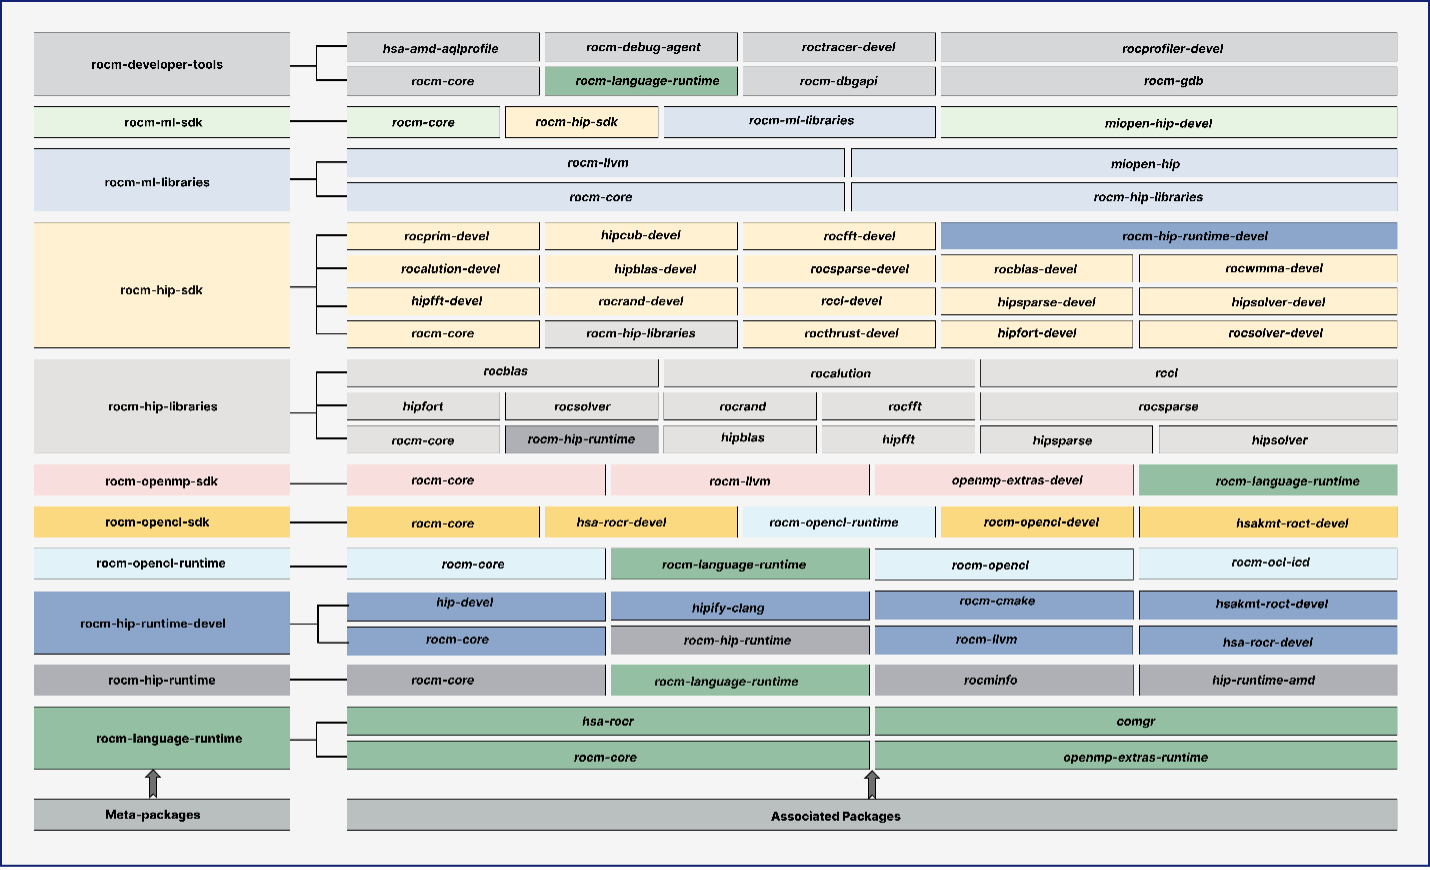
\includegraphics[width=1\linewidth]{Appendici/MetaPackages.png}
    \caption{ROCm 元套件的列表以及包含在元套件中的各個獨立套件}
    \label{fig:rocm_packages}
\end{figure}


\section{安裝}

在此概論中,我們介紹兩種安裝 ROCm 的方法,包含安裝程式腳本的方法與套件管理器的方法。

\subsection{安裝程式腳本方法}
\label{sec:rocm_installer_method}
安裝程式腳本方法自動化了 AMDGPU 和 ROCm 的安裝過程。安裝程式腳本會處理 ROCm 的完整安裝過程,包括設定儲存庫、清理檔案系統、更新和安裝所需的驅動程式與元套件。使用此方法,系統對 ROCm 安裝過程有更多控制權。因此,那些對標準 Linux 指令不太熟悉的使用者可以選擇此方法來安裝 ROCm。可以使用以下指令下載並安裝安裝程式:

\begin{lstlisting}[caption={使用安裝程式腳本安裝 ROCm 所需指令}, label={lst:a1}]
sudo apt-get update
wget https://repo.radeon.com/amdgpu-install/5.4.3/ubuntu/focal/amdgpu-install_5.4.50403-1_all.deb
sudo apt-get install ./amdgpu-install_5.4.50403-1_all.deb
\end{lstlisting}

上述指令應該會安裝一個可以幫助管理 ROCm 套件的 \lstinline|amdgpu-install| 程式。如要安裝 ROCm,我們可以使用 \lstinline|sudo ./amdgpu-install| 指令執行安裝。此外,使用者也可以透過像是 \lstinline|sudo amdgpu-install --usecase=rocm| 的指令來安裝特定的使用案例。如果使用者希望一次安裝多個使用案例,可以在 \lstinline|usecase| 參數中指定多個值,並以逗號分隔。例如,指令 \lstinline|sudo amdgpu-install --usecase=rocm,hiplibsdk| 會同時安裝 ROCm 和 \lstinline|hiplibsdk| 兩個使用案例。使用 \lstinline|sudo amdgpu-install --list-usecase| 可以顯示所有可用的使用案例的列表。


\subsection{套件管理器方法}

套件管理器方法提供使用者更多安裝選項的靈活性,但在安裝過程中需要更多的使用者操作。建議此方法僅供進階使用者使用。總體來說,使用套件管理器安裝 ROCm 包括以下六個步驟:

\paragraph{步驟 1:安裝 Linux 核心標頭與開發套件}
使用套件管理器方法的前置步驟之一是安裝正確的 Linux 核心標頭與開發套件。

可以使用指令 \lstinline!sudo dpkg -l | grep linux-headers! 來檢查已安裝的核心標頭版本。例如,輸出的結果可能是 \lstinline|ii linux-headers-5.15.0-41-generic 5.15.0-41.44 20.04.1 amd64 Linux kernel headers for version 5.15.0 on 64 bit x86 SMP|。
類似地,可以使用指令 \lstinline!sudo dpkg -l | grep linux-modules-extra! 來列出開發套件,在作者的系統中輸出的結果為
\lstinline|ii linux-modules-extra-5.15.0-41-generic 5.15.0-41.44 20.04.1 amd64 Linux kernel extra modules for version 5.15.0 on 64 bit x86 SMP|。
如果當前版本的 Linux 標頭不符合表 \ref{table:rocm_supported_distros_and_kernel_versions} 中列出的要求,使用者需要使用指令 \lstinline|sudo apt install linux-headers-$(uname -r) linux-modules-extra-$(uname -r)| 來安裝所需的 Linux 標頭。


\paragraph{步驟 2:安裝 AMD GPU 驅動程式}
接下來,我們會使用套件管理器安裝 AMD GPU 驅動程式。套件管理器要求套件必須加密,因此需要安裝一組 GNU Privacy Guard(GPG)金鑰。安裝 GPG 金鑰的指令為:

\lstinline!curl -fsSL https://repo.radeon.com/rocm/rocm.gpg.key | sudo gpg --dearmor -o /etc/apt/trusted.gpg.d/rocm-keyring.gpg!。

接下來,使用以下指令將 AMD GPU 儲存庫新增到 Ubuntu 的套件管理器中:

\lstinline!echo 'deb [arch=amd64 signed-by=/etc/apt/trusted.gpg.d/rocm-keyring.gpg] https://repo.radeon.com/amdgpu/5.4.3/ubuntu focal main' | sudo tee /etc/apt/sources.list.d/amdgpu.list!。
新增儲存庫後,別忘了執行 \lstinline|sudo apt-get update|,讓套件管理器能夠取得套件資訊。
最後,使用 \lstinline|sudo apt install amdgpu-dkms| 來安裝 AMD GPU 驅動程式。安裝完成後,需要重新啟動系統。

\paragraph{步驟 3:安裝 ROCm 環境}
為了安裝 ROCm 環境,我們需要使用以下指令將外部資源加入到 Ubuntu 的套件管理器中:

\lstinline!echo 'deb [arch=amd64 signed-by=/etc/apt/trusted.gpg.d/rocm-keyring.gpg] https://repo.radeon.com/rocm/apt/5.4.3 focal main' | sudo tee /etc/apt/sources.list.d/rocm.list!

此指令會建立 \lstinline|rocm.list|,其中包含提供套件的 URL。

接下來,我們需要透過以下指令修改優先權:

\lstinline!echo -e 'Package: *\nPin: release o=repo.radeon.com\nPin-Priority: 600' | sudo tee /etc/apt/preferences.d/rocm-pin-600! 

透過為 ROCm 套件設定較高的優先權,我們可以在更新套件時保持穩定版本的 Ubuntu。在新增套件來源並修改優先設定後,我們仍然需要執行 \lstinline|sudo apt-get update|。


\subsection{驗證安裝}
無論使用哪種安裝方法,我們都需要驗證安裝是否成功。如果執行過程中出現錯誤,使用者應該首先檢查 ROCm 安裝是否已損壞。

首先,我們可以檢查 \lstinline|/opt/rocm|目錄是否包含預期的執行檔,例如 \lstinline|rocm-smi|,以及 ROCm 函式庫,例如 \lstinline|librocblas.so|。
其次,我們可以檢查驅動程式是否正常運作。可以使用 \lstinline|dkms status| 指令檢查目前正在使用的驅動程式。例如,在作者的系統中,執行此指令會顯示輸出:\lstinline|amdgpu, 5.16.9.22.20-1438746~20.04, 5.4.0-121-generic, x86_64: installed|。這表示驅動程式已正確安裝並正在使用。

再來,我們應該檢查是否有程式能夠偵測到 GPU 硬體並取得 GPU 的屬性。我們可以執行 \lstinline|/opt/rocm/bin/rocminfo| 或 \lstinline|/opt/rocm/opencl/bin/clinfo| 來取得硬體屬性。如果這兩個程式能夠順利執行並且顯示系統中安裝的 GPU,則表示 ROCm 環境已正確安裝並且正常運作。

最後,我們可以使用平常的 Ubuntu 套件安裝指令來安裝元套件。指令為 \lstinline|sudo apt install <套件名稱>|。例如,如果我們想安裝最常使用的 ROCm 功能,可以使用 \lstinline|sudo apt install rocm|。


\section{更新 ROCm}
保持新版本的 ROCm 非常重要,因為工具和函式庫會不斷收到新的功能更新、錯誤修復、效能改善和安全性更新。和安裝過程類似,使用者可以選擇使用安裝程式或是 Linux 發行版提供的套件管理器。

若要使用安裝程式腳本方法,首先需要按照章節 \ref{sec:rocm_installer_method} 所描述的步驟安裝安裝程式。接下來,升級套件版本的過程與全新安裝相同。若要更新特定的使用案例,可以使用指令 \lstinline|sudo amdgpu-install --usecase=<使用案例>|。

若是使用套件管理器更新 ROCm,則會需要較多指令。首先,我們需要更新 AMD GPU 驅動程式套件的外部來源,使用以下指令:

\lstinline!echo 'deb [arch=amd64 signed-by=/etc/apt/trusted.gpg.d/rocm-keyring.gpg] <amdgpu baseurl> focal main' | sudo tee /etc/apt/sources.list.d/amdgpu.list!

修改來源清單後需要執行 \lstinline|sudo apt-get update|。接著,我們可以使用指令 \lstinline|sudo apt install amdgpu-dkms| 來更新驅動程式。同樣,安裝完成後,需要重新啟動系統。

最後,我們需要對 ROCm 套件重複此過程。使用以下指令來修改外部來源:

\lstinline!echo 'deb [arch=amd64 signed-by=/etc/apt/trusted.gpg.d/rocm-keyring.gpg] <rocm baseurl> focal main' | sudo tee /etc/apt/sources.list.d/rocm.list!

\lstinline!echo -e 'Package: *\nPin: release o=repo.radeon.com\nPin-Priority: 600' | sudo tee /etc/apt/preferences.d/rocm-pin-600!

接著,我們可以使用套件管理器更新 ROCm 套件,指令為:\lstinline|sudo apt install --only-upgrade <套件名稱>|。

\section{解除安裝 ROCm}
若要解除安裝 ROCm,我們可以選擇使用安裝程式腳本(在這種情況下是解除安裝程式)或是 Linux 發行版的套件管理器。如果 ROCm 是透過安裝程式腳本安裝的,解除安裝程式會與安裝程式一併提供。解除安裝 ROCm 只需執行 \lstinline|sudo amdgpu-uninstall| 即可。
Ubuntu 的套件管理器可以輕鬆解除安裝 ROCm 或特定的使用案例。指令為:
\lstinline|sudo apt autoremove <套件名稱>|。


\begin{table}[h!]
\centering
\caption{ROCm 的元套件}
\label{table:rocm_meta_packages}
\begin{tabular}{lp{0.6\linewidth}}
\hline
\textbf{元套件}               & \textbf{說明}  \\
\hline
\lstinline|rocm-hip-libraries|            & \lstinline|rocm-hip-libraries| 會安裝為 AMD 平台優化的 HIP 函式庫。                                            \\
\lstinline|rocm-hip-runtime|              & \lstinline|rocm-hip-runtime| 會安裝運行在 AMD 平台上以 HIP 撰寫的應用程式所需的套件            \\
\lstinline|rocm-hip-runtime-devel|        & \lstinline|rocm-hip-runtime-devel| 會安裝開發基於 HIP 的應用程式或將其從 CUDA 移植過來所需的套件   \\
\lstinline|rocm-hip-sdk|                  & \lstinline|rocm-hip-sdk| 會安裝開發/移植使用 HIP 的應用程式所需的套件以及為 AMD 平台提供的函式庫  \\
\lstinline|rocm-language-runtime|         & \lstinline|rocm-language-runtime| 會安裝 ROCm 執行環境   \\
\lstinline|rocm-ml-libraries|             & \lstinline|rocm-ml-libraries| 會安裝關鍵的機器學習函式庫套件(主要是 MIOpen)  \\
\lstinline|rocm-ml-sdk|                   & \lstinline|rocm-ml-sdk| 會安裝開發和運行使用為 AMD 平台優化的機器學習運算單元的應用程式所需的套件  \\
\lstinline|rocm-opencl-runtime|           & \lstinline|rocm-opencl-runtime| 會安裝在 AMD 平台上執行基於 OpenCL 的應用程式所需的套件   \\
\lstinline|rocm-opencl-sdk|               & \lstinline|rocm-opencl-sdk| 會安裝在 AMD 平台上開發基於 OpenCL 的應用程式所需的套件  \\
\lstinline|rocm-openmp-runtime|           & \lstinline|rocm-openmp-runtime| 會安裝在 AMD 平台上執行基於 OpenMP 的應用程式所需的套件  \\
\lstinline|rocm-openmp-sdk|               & \lstinline|rocm-openmp-sdk| 會安裝在 AMD 平台上開發基於 OpenMP 的應用程式所需的套件   \\
\hline
\end{tabular}
\end{table}


%%%%%%%%%%%%%%%%%%%%%%%%%%%%									BACKMATTER
%%%%%%%%%%%%%%%%%%%%%%%%%%%%
\backmatter

%%%%% 							BIBLIOGRAFIA
\pagestyle{fancyBibliografia}
\titleformat{\chapter}
	[hang]
	{\vspace{-2cm}\Huge}
	{}
	{0em}
	{}
	[\Large {\begin{tikzpicture} [remember picture, overlay]
	\pgftext[right,x=14.75cm,y=0.2cm]{\HUGE\bfseries 
	Bibliografia}
	\end{tikzpicture}}]
	
	\nocite{*}
	\bibliographystyle{amsalpha}
	\bibliography{FileAusiliari/Bibliografia}
	\addcontentsline{toc}{part}{Bibliografia}
\cleardoublepage
%INDICE ANALITICO
 \pagestyle{fancyIndiceAnalitico}
 	\renewcommand{\indexname}{}
	% SISTEMA IL PROBLEMA DEL LINK ALL'INDICE ANALITICO
	\let\cleardoublepage\relax
	\titleformat{\chapter}[hang]{}{}{0em}{}[]
 	\chapter*{}
	\titleformat{\chapter}
		[hang]
		{\Huge}
		{}
		{0em}
		{}
		[\Large {\begin{tikzpicture} [remember picture, overlay]
		\pgftext[right,x=14.75cm,y=0.2cm]{\HUGE\bfseries 
			Indice analitico}
		\end{tikzpicture}}]
	\titlespacing*{\chapter}{0pt}{0\baselineskip}{5\baselineskip}
	\addcontentsline{toc}{part}{Indice analitico}	
	\vspace{-2cm}
	\printindex
%%%%%%%%%%%%%%%%%%%%%%%%%%%%%%%%%%%%%%%%%%%%%%%%%%%%%%%%%%%%%%%%%%%%%%%%%%%%%%%%%%%%%%%%%%%%%%%%%%%%%%%%%%%%%%%%%
\end{appendices}
\end{document}